\documentclass[11pt,]{article}
\usepackage[left=1in,top=1in,right=1in,bottom=1in]{geometry}
\newcommand*{\authorfont}{\fontfamily{phv}\selectfont}
\usepackage[]{mathpazo}


  \usepackage[T1]{fontenc}
  \usepackage[utf8]{inputenc}




\usepackage{abstract}
\renewcommand{\abstractname}{}    % clear the title
\renewcommand{\absnamepos}{empty} % originally center

\renewenvironment{abstract}
 {{%
    \setlength{\leftmargin}{0mm}
    \setlength{\rightmargin}{\leftmargin}%
  }%
  \relax}
 {\endlist}

\makeatletter
\def\@maketitle{%
  \newpage
%  \null
%  \vskip 2em%
%  \begin{center}%
  \let \footnote \thanks
    {\fontsize{18}{20}\selectfont\raggedright  \setlength{\parindent}{0pt} \@title \par}%
}
%\fi
\makeatother




\setcounter{secnumdepth}{0}

\usepackage{longtable,booktabs}



\title{Predicting Property Prices: A Machine Learning Approach  }



\author{\Large Albina Cako, BSc\vspace{0.05in} \newline\normalsize\emph{York University, Certificate in Machine Learning}   \and \Large Colin Green, BSc\vspace{0.05in} \newline\normalsize\emph{York University, Certificate in Machine Learning}   \and \Large Lucy Zhang, BSc\vspace{0.05in} \newline\normalsize\emph{York University, Certificate in Machine Learning}   \and \Large Sean X. Zhang, MSc\vspace{0.05in} \newline\normalsize\emph{York University, Certificate in Machine Learning}  }


\date{}

\usepackage{titlesec}

\titleformat*{\section}{\normalsize\bfseries}
\titleformat*{\subsection}{\normalsize\itshape}
\titleformat*{\subsubsection}{\normalsize\itshape}
\titleformat*{\paragraph}{\normalsize\itshape}
\titleformat*{\subparagraph}{\normalsize\itshape}





\newtheorem{hypothesis}{Hypothesis}
\usepackage{setspace}


% set default figure placement to htbp
\makeatletter
\def\fps@figure{htbp}
\makeatother

\usepackage{hyperref}
\usepackage{subfig}
\usepackage{booktabs}
\usepackage{longtable}
\usepackage{array}
\usepackage{multirow}
\usepackage{wrapfig}
\usepackage{float}
\usepackage{colortbl}
\usepackage{pdflscape}
\usepackage{tabu}
\usepackage{threeparttable}
\usepackage{threeparttablex}
\usepackage[normalem]{ulem}
\usepackage{makecell}
\usepackage{xcolor}

% move the hyperref stuff down here, after header-includes, to allow for - \usepackage{hyperref}

\makeatletter
\@ifpackageloaded{hyperref}{}{%
\ifxetex
  \PassOptionsToPackage{hyphens}{url}\usepackage[setpagesize=false, % page size defined by xetex
              unicode=false, % unicode breaks when used with xetex
              xetex]{hyperref}
\else
  \PassOptionsToPackage{hyphens}{url}\usepackage[draft,unicode=true]{hyperref}
\fi
}

\@ifpackageloaded{color}{
    \PassOptionsToPackage{usenames,dvipsnames}{color}
}{%
    \usepackage[usenames,dvipsnames]{color}
}
\makeatother
\hypersetup{breaklinks=true,
            bookmarks=true,
            pdfauthor={Albina Cako, BSc (York University, Certificate in Machine Learning) and Colin Green, BSc (York University, Certificate in Machine Learning) and Lucy Zhang, BSc (York University, Certificate in Machine Learning) and Sean X. Zhang, MSc (York University, Certificate in Machine Learning)},
             pdfkeywords = {house prices, machine learning, caret, shiny},  
            pdftitle={Predicting Property Prices: A Machine Learning Approach},
            colorlinks=true,
            citecolor=blue,
            urlcolor=blue,
            linkcolor=magenta,
            pdfborder={0 0 0}}
\urlstyle{same}  % don't use monospace font for urls

% Add an option for endnotes. -----


% add tightlist ----------
\providecommand{\tightlist}{%
\setlength{\itemsep}{0pt}\setlength{\parskip}{0pt}}

% add some other packages ----------

% \usepackage{multicol}
% This should regulate where figures float
% See: https://tex.stackexchange.com/questions/2275/keeping-tables-figures-close-to-where-they-are-mentioned
\usepackage[section]{placeins}


\begin{document}
	
% \pagenumbering{arabic}% resets `page` counter to 1 
%
% \maketitle

{% \usefont{T1}{pnc}{m}{n}
\setlength{\parindent}{0pt}
\thispagestyle{plain}
{\fontsize{18}{20}\selectfont\raggedright 
\maketitle  % title \par  

}

{
   \vskip 13.5pt\relax \normalsize\fontsize{11}{12} 
\textbf{\authorfont Albina Cako, BSc} \hskip 15pt \emph{\small York University, Certificate in Machine Learning}   \par \textbf{\authorfont Colin Green, BSc} \hskip 15pt \emph{\small York University, Certificate in Machine Learning}   \par \textbf{\authorfont Lucy Zhang, BSc} \hskip 15pt \emph{\small York University, Certificate in Machine Learning}   \par \textbf{\authorfont Sean X. Zhang, MSc} \hskip 15pt \emph{\small York University, Certificate in Machine Learning}   

}

}








\begin{abstract}

    \hbox{\vrule height .2pt width 39.14pc}

    \vskip 8.5pt % \small 

\noindent The project focuses on building a machine learning model to predict
house prices in Toronto. The training dataset contained 15234 sold
listings between 2018 and 2019. The model was based on 6 features: area
(in square feet), mean distrinct income, number of bedrooms, number of
bathrooms, number of parking spaces and property type. We evaluated four
different machine-learning models and chose XGBoost as the most accurate
model. A Shiny app was then created to predict the estimated listing and
final prices.


\vskip 8.5pt \noindent \emph{Keywords}: house prices, machine learning, caret, shiny \par

    \hbox{\vrule height .2pt width 39.14pc}



\end{abstract}


\vskip -8.5pt


 % removetitleabstract

\noindent  

\hypertarget{introduction}{%
\section{Introduction}\label{introduction}}

Purchasing a property is often an important life decision for every
individual and requires a considerable amount of research. Buying a home
holds many different purposes, whether it is for dwelling or as a future
investment. Also, selling a house requires significant research to
decide the optimal listing price. Commonly, people will seek advice from
various websites or real estate agents before purchasing; however, due
to big data trends, house price prediction can be also done by using
machine learning strategies based on large datasets from previous years.
House Price Index (HPI) can measure the price changes of residential
housing as a percentage change. In Canada, the new Housing Price Index
is calculated monthly by Statistics Canada. HPI is useful, however, it
does not give a precise estimate of any specific house with its own
attributes {[}1{]}. The objective of this project was to evaluate the
application of several machine learning algorithms to predict house
prices in the City of Toronto using their attributes and location.

The House Pricing Prediction app was created to estimate both the final
and list prices, so it can be used by buyers and sellers. The deployment
was constructed using ShinyApp and it used the houses' locations and
attributes. The app can be used for individual buyers who want to know
the final price of the houses they are interested in or for individual
sellers to know what the best listing price is. This project used
regression and comprehensively validated four different machine learning
models: decision tree, random forest, gradient boosting machine and
XGBoost. The models were tuned and the XGBoost was chosen for deployment
for its high accuracy. In this report we present the full process of
data visualization, cleaning and manipulation, as well as feature
selection, model training, model tuning and deployment on ShinyApp.

\hypertarget{methodology}{%
\section{Methodology}\label{methodology}}

\hypertarget{data-preprocessing}{%
\subsection{Data Preprocessing}\label{data-preprocessing}}

The housing dataset, originally shared on Github {[}2{]}, was extracted
from Zoocasa.com in 2019. The dataset contains all completed property
sales in the city of Toronto within a 1-year span between 2018-2019. We
performed several data exploration and cleaning steps to prepare the
dataset for modeling.

\hypertarget{missingness}{%
\subsection{Missingness}\label{missingness}}

We assessed the dataset for missing values, as missing data often
introduce bias and reduce accuracy in machine learning models {[}3{]}.
Thus, missing values ought to be either imputed or removed before data
modeling. We then determined whether missing data was Missing Completely
at Random (MCAR), Missing at Random (MAR), or Missing Not at Random
(MNAR). Should the data be MCAR, then it is acceptable to simply remove
each observation that is missing, as doing so would not introduce bias
to the remaining observations. However, if there was a correlation
between missingness and other data features, then imputation must be
performed {[}4{]}. Missingness correlation was assessed using the
missing\_compare() function from the finalfit library, which applies the
Kruskal Wallis correlation test for numerical variables and Chi-squared
correlation test for categorical variables to determine correlation
{[}5{]}. Using the MICE package in R, we then applied the following
imputation methods: 1) simple, which imputes a value from a simple
random sample from the rest of the data; 2) mean, which imputes the
average of all observations; 3) random forest, which applies a random
forest algorithm; and 4) CART, which imputes by classification and
regression trees. The distribution of the imputed data were evaluated
with a density plot and an imputed dataset was chosen based on best fit
{[}6{]}.

\hypertarget{assessing-parametric-fit}{%
\subsection{Assessing Parametric Fit}\label{assessing-parametric-fit}}

Outliers were visualized with the boxplot() function. Data were
considered outliers if they were less than Q1 - 1.5 X Inter-Quartile
Range and greater Q3 + 1.5 X Inter-Quartile Range. Normality of the
distribution of variables were visualized with density plots. A
correlogram with Pearson's coefficient determined collinearity. Linear
relationship between outcome variable and predictors was tested via
scatterplots.

\hypertarget{data-curation}{%
\subsection{Data Curation}\label{data-curation}}

The following variables were removed as they did not have any data
utility or were not easily parseable (i.e.~free text): title,
description, mls, type, full\_link, full\_address. A numeric `bedrooms'
column was created by combining bedrooms\_ag and bedrooms\_bg. We also
removed district\_code and city\_district. Both were categorical
variables with number of factors = 140; keeping these would
significantly increase model training time {[}7{]}. We also did not
consider longitude and latitude, as including these variables in
training sets would have required geocoding and district clustering;
complexities which were outside our scope for this application.
Mean\_district\_income was left as an approximation of the effect of
districts on property price. After consultation with a real-estate
expert, we decreased the number of property types by generalizing types
to: Townhouse, Condo, Detached, Semi-Detached, and Plex. Thus, the
predictors chosen were:

\begin{longtable}[]{@{}lll@{}}
\caption{Predictor variables}\tabularnewline
\toprule
Variable & & Type\tabularnewline
\midrule
\endfirsthead
\toprule
Variable & & Type\tabularnewline
\midrule
\endhead
sqft & & numeric\tabularnewline
beds & & numeric\tabularnewline
bathrooms & & numeric\tabularnewline
parking & & numeric\tabularnewline
mean\_district\_income & & numeric\tabularnewline
type & & categorical\tabularnewline
\bottomrule
\end{longtable}

We chose final\_price as the target variable. While the dataset also
contained a list\_price variable, rather than training two models to
predict on both list and final price, the predicted list price was
instead approximated by a linear equation between list and final price
from the original dataset.

\hypertarget{modeling}{%
\subsection{Modeling}\label{modeling}}

The data contained a mix of categorical and numerical variables. These
variables did not satisfy the many requirements of parametric models,
such as variable independence, normally distributed data, and linear
relationship with outcome {[}8{]}. Thus, several non-parametric models
were used instead. We trained four different models using k-fold cross
validation. The models were then tuned using various grid searches to
improve the accuracy. The final model was then chosen based on three
accuracy metrics: Root Mean-Squared Error (RMSE), Pearson correlation
(\(R^2\)), and Mean Average Error (MAE).

\begin{longtable}[]{@{}lll@{}}
\caption{Non-parametric Models Used}\tabularnewline
\toprule
\begin{minipage}[b]{0.08\columnwidth}\raggedright
Model\strut
\end{minipage} & \begin{minipage}[b]{0.63\columnwidth}\raggedright
Description\strut
\end{minipage} & \begin{minipage}[b]{0.21\columnwidth}\raggedright
Tuning parameters\strut
\end{minipage}\tabularnewline
\midrule
\endfirsthead
\toprule
\begin{minipage}[b]{0.08\columnwidth}\raggedright
Model\strut
\end{minipage} & \begin{minipage}[b]{0.63\columnwidth}\raggedright
Description\strut
\end{minipage} & \begin{minipage}[b]{0.21\columnwidth}\raggedright
Tuning parameters\strut
\end{minipage}\tabularnewline
\midrule
\endhead
\begin{minipage}[t]{0.08\columnwidth}\raggedright
Decision Tree\strut
\end{minipage} & \begin{minipage}[t]{0.63\columnwidth}\raggedright
Decision trees repeatedly partition data at specific nodes until the
data at the bottom of each branch (known as a leaf) is as homogenous as
possible. The model increases in complexity with each additional
partition and subsequently becomes more accurate {[}9{]}.\strut
\end{minipage} & \begin{minipage}[t]{0.21\columnwidth}\raggedright
cp (complexity)\strut
\end{minipage}\tabularnewline
\begin{minipage}[t]{0.08\columnwidth}\raggedright
Random Forest\strut
\end{minipage} & \begin{minipage}[t]{0.63\columnwidth}\raggedright
Random Forest Model Random Forests are an ensemble learning method for
classification and regression. This method will construct a multitude of
decision trees and output the mean/average prediction problem for
regression or the classes for classification problem. The algorithm can
control the number of variable available for splitting at each tree or
the number of trees to get a higher accuracy {[}10{]}.\strut
\end{minipage} & \begin{minipage}[t]{0.21\columnwidth}\raggedright
ntree, mtry\strut
\end{minipage}\tabularnewline
\begin{minipage}[t]{0.08\columnwidth}\raggedright
Gradient Boosting Machines\strut
\end{minipage} & \begin{minipage}[t]{0.63\columnwidth}\raggedright
Gradient Boosting Machines (gbm) begin with creating a preliminary `weak
learner' decision tree, then sequentially grows more trees that aim to
reduce the error of the last one. The algorithm optimizes the loss
function by minimizing the residuals at each iteration (difference
between predicted and actual value) {[}11{]}.\strut
\end{minipage} & \begin{minipage}[t]{0.21\columnwidth}\raggedright
n.trees, shrinkage, interaction.depth, n.minobssinnode\strut
\end{minipage}\tabularnewline
\begin{minipage}[t]{0.08\columnwidth}\raggedright
XGBoost\strut
\end{minipage} & \begin{minipage}[t]{0.63\columnwidth}\raggedright
XGBoost uses ensemble learning, which is a systematic solution that
combines the predictive power of multiple learners. It outputs a single
model that gives the combined output from many models. This allows the
opportunity to not rely on the results of a single machine learning
model. In this particular model, the trees are built sequentially, such
that the next tree focuses on reducing the errors of the previous tree
{[}12{]}.\strut
\end{minipage} & \begin{minipage}[t]{0.21\columnwidth}\raggedright
nrounds, max\_depth, eta, gamma, colsample\_bytree, min\_child\_weight,
subsample\strut
\end{minipage}\tabularnewline
\bottomrule
\end{longtable}

\hypertarget{deployment}{%
\subsection{Deployment}\label{deployment}}

The application was created using R shiny and hosted on the Shinyapps.io
cloud. Districts were plotted using mean latitude and longitude of all
properties from the housing dataset. Some districts had few properties
to create a centroid from; these were manually fixed using geographic
data extracted from Toronto neighborhood websites {[}13{]}{[}14{]}.

\hypertarget{results}{%
\section{Results}\label{results}}

The original housing dataset contained 21 variables and 15234
observations. Table 1 defines each variable of the dataset.
\hyperref[sec:map]{Figure 1} plots the geographic distribution of
properties based on long/lat.

\begin{longtable}[]{@{}lll@{}}
\caption{Data Dictionary}\tabularnewline
\toprule
Variable & & Type\tabularnewline
\midrule
\endfirsthead
\toprule
Variable & & Type\tabularnewline
\midrule
\endhead
title & & Title of the listing\tabularnewline
final\_price & & Final price of the property\tabularnewline
list\_price & & Listing price of the property\tabularnewline
bedrooms & & Number of bedrooms\tabularnewline
bathrooms & & Number of bathrooms\tabularnewline
sqft & & Area of property in square feet\tabularnewline
parking & & Number of parking spaces\tabularnewline
description & & Verbatim text description of the property\tabularnewline
mls & & MLS Listing ID\tabularnewline
type & & Property type\tabularnewline
full\_link & & URL to listing\tabularnewline
full\_address & & Full address of the property\tabularnewline
lat & & Latitude\tabularnewline
long & & Longitude\tabularnewline
city\_district & & Toronto district to which property belonged
to\tabularnewline
mean\_district\_income & & Average household income of
district\tabularnewline
district\_code & & Numerical code of the district\tabularnewline
final\_price\_transformed & & Box-Cox transformation of final
price\tabularnewline
final\_price\_log & & Log transformation of final price\tabularnewline
bedrooms\_ag & & Number of bedrooms above ground\tabularnewline
bedrooms\_bg & & Number of bedrooms below ground\tabularnewline
\bottomrule
\end{longtable}

\hypertarget{data-exploration}{%
\subsection{Data Exploration}\label{data-exploration}}

The mean final price property price in Toronto between 2018 and 2019 was
\$715,000, with a median number of 3 bedrooms and 2 bathrooms. The most
common properties types were condo (58.2\%), detached (28.8\%), and
semi-detached (9.4\%).

\begin{verbatim}
##   final_price          bedrooms        bathrooms           sqft     
##  Min.   :  103000   Min.   : 0.000   Min.   : 1.000   Min.   : 250  
##  1st Qu.:  535000   1st Qu.: 2.000   1st Qu.: 1.000   1st Qu.: 650  
##  Median :  715000   Median : 3.000   Median : 2.000   Median : 900  
##  Mean   :  882714   Mean   : 2.875   Mean   : 2.122   Mean   :1116  
##  3rd Qu.:  989000   3rd Qu.: 4.000   3rd Qu.: 3.000   3rd Qu.:1300  
##  Max.   :13180000   Max.   :14.000   Max.   :14.000   Max.   :4374  
##                                                       NA's   :4521  
##     parking       mean_district_income
##  Min.   : 0.000   Min.   : 25989      
##  1st Qu.: 1.000   1st Qu.: 34904      
##  Median : 1.000   Median : 50580      
##  Mean   : 1.559   Mean   : 56066      
##  3rd Qu.: 2.000   3rd Qu.: 67757      
##  Max.   :11.000   Max.   :308010      
## 
\end{verbatim}

\begin{verbatim}
## 
##         Condo      Detached          Plex Semi-Detached     Townhouse 
##          8874          4388            70          1435           467
\end{verbatim}

\begin{figure}

{\centering 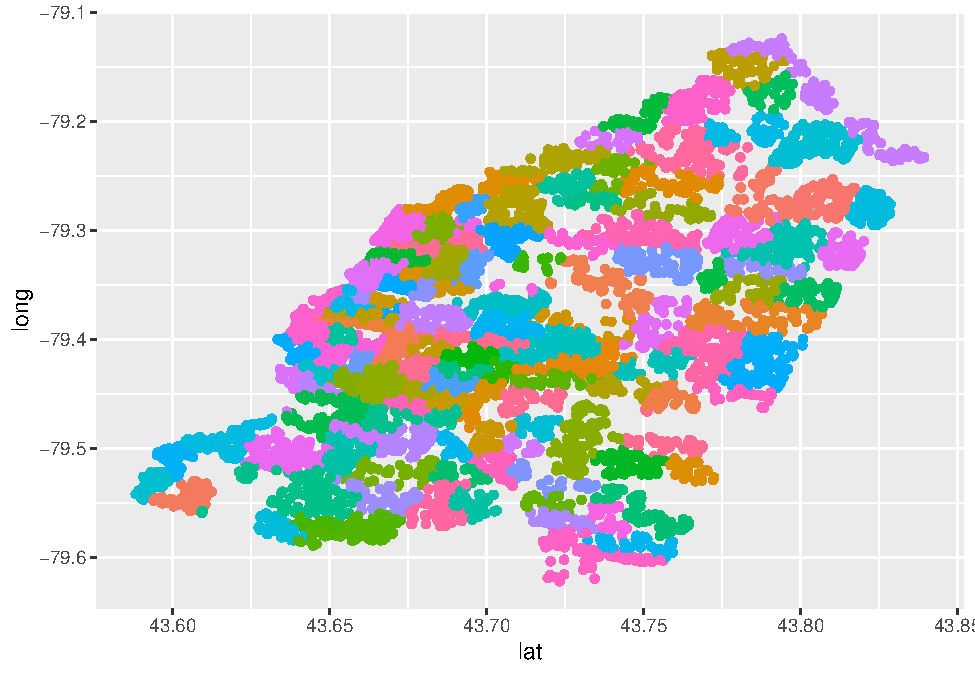
\includegraphics{R-markdown_sean_files/figure-latex/map-1} 

}

\caption{Geographic Distribution of Property Data\label{sec:map}}\label{fig:map}
\end{figure}

The `sqft' variable was missing 4315 observations (30\%). To test
whether the missing data was MCAR, we compared whether other variables
were associated with missingness. Using Chi-squared and Kruskal Wallis
tests for categorical and numerical variables, respectively, we
determined that housing and price had significant correlation
(p\textless0.01) with sqft missingness, where properties missing sqft
trended towards higher prices. Thus, we conclude that sqft is not MCAR,
so we cannot simply remove observations where sqft is missing without
introducing bias. To account for missing values, we chose to use the
CART (Classification and Regression Trees) method of imputation
(\hyperref[sec:fig2]{Figure 2}). Blue represents the distribution of the
original data, while red represents the distribution of imputed data.
The mean sqft increased from 1116 to 1311 as a result of the imputation.

\begin{verbatim}
##    Min. 1st Qu.  Median    Mean 3rd Qu.    Max. 
##     250     750    1100    1311    1750    4374
\end{verbatim}

\begin{figure}

{\centering 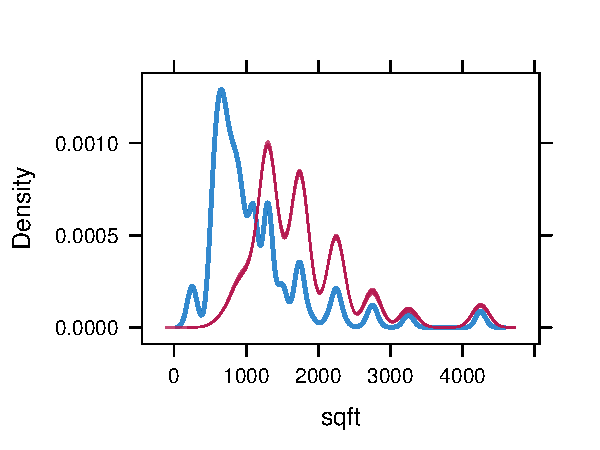
\includegraphics{R-markdown_sean_files/figure-latex/CART imputation-1} 

}

\caption{CART-imputed values for sqft\label{sec:fig2}}\label{fig:CART imputation}
\end{figure}

We then performed a correlation analysis based on Pearson's coefficient
between each numeric predictor. We considered a correlation
\textgreater{} 0.5, with p \textless{} 0.05 as a significant
correlation. \hyperref[sec:fig3]{Figure 3} demonstrates significant
correlation between many of our predictor variables.

\begin{figure}

{\centering 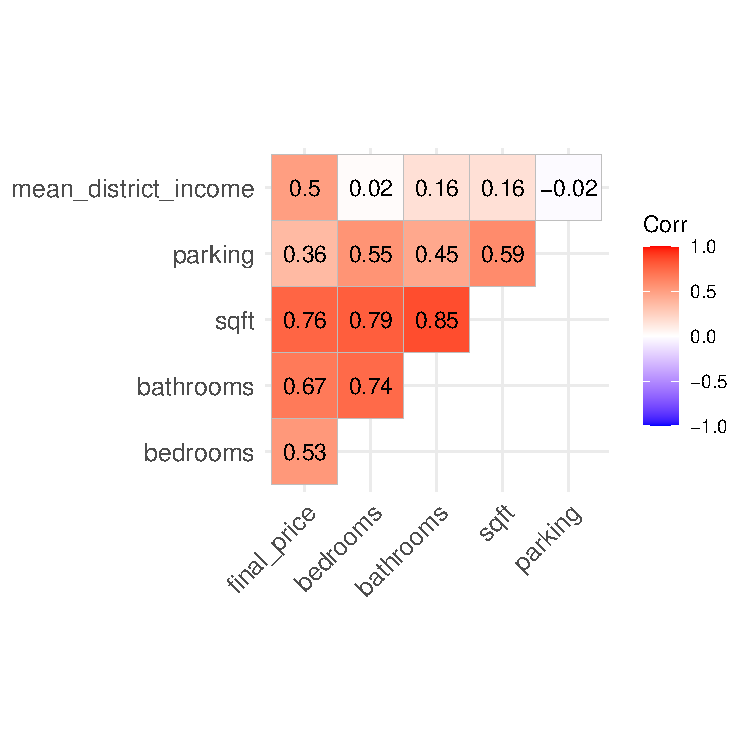
\includegraphics{R-markdown_sean_files/figure-latex/corrplot-1} 

}

\caption{Correlogram\label{sec:fig3}}\label{fig:corrplot}
\end{figure}

We also summarize the distribution of predictor and target variables
(\hyperref[sec:fig4]{Figure 4}). Note the right skew in each predictor
variable as well as amount of outliers in each of our predictor
variables. Finally, we checked for whether a linear relationship existed
between each predictor variables and the target variable
(\hyperref[sec:fig5]{Figure 5}). Overall, the data is unlikely to be
well-fit for parametric machine-learning algorithms such as generalized
linear regression. The data does not satisfy the assumptions of variable
independence, normal distribution, nor a linear relationship between
predictors and target variable. Thus, we chose to use non-parametric
algorithms to model our data instead.

\begin{figure}

{\centering 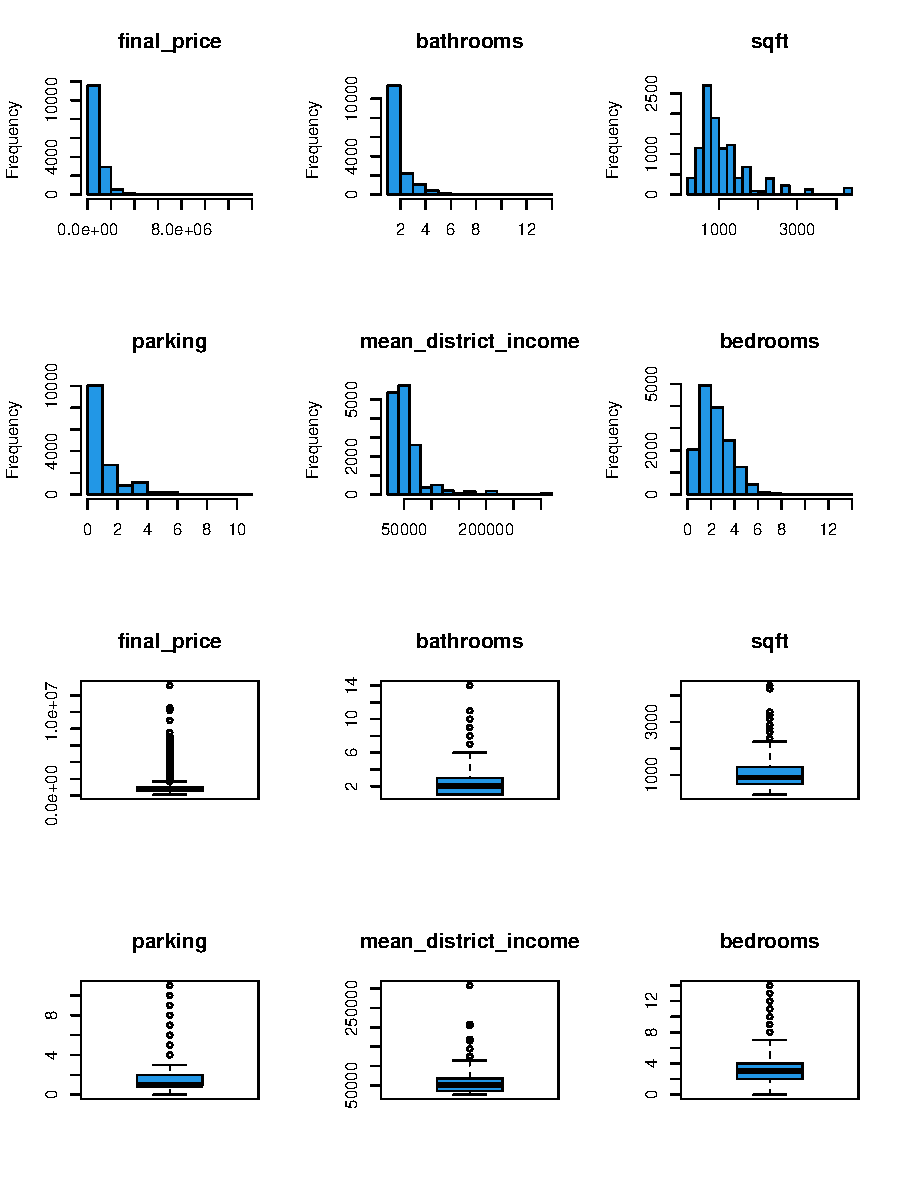
\includegraphics{R-markdown_sean_files/figure-latex/histogram-1} 

}

\caption{Distribution of predictor and target variables\label{sec:fig4}}\label{fig:histogram}
\end{figure}
\begin{figure}

{\centering 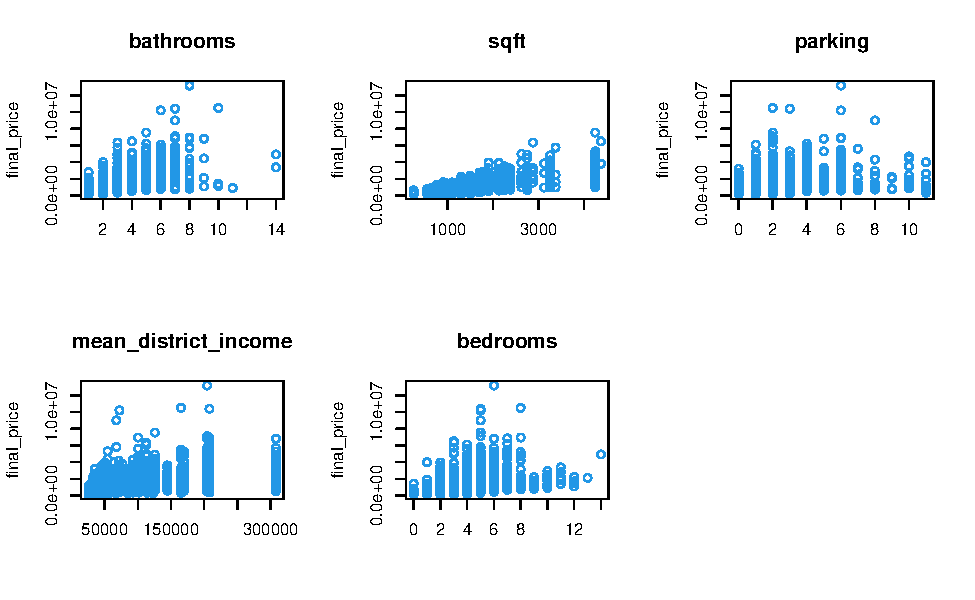
\includegraphics{R-markdown_sean_files/figure-latex/linear correlation-1} 

}

\caption{Scatterplot of Predictors vs. Final Price\label{sec:fig5}}\label{fig:linear correlation}
\end{figure}

We chose final\_price as our target variable, but still wished to
include list\_price in the deployment of our application. Therefore, the
list price is predicted via the following linear regression
(\hyperref[sec:fig6]{Figure 6}):
\[list\_price = 1.032594 * final\_price - 36525.78\]

\begin{figure}

{\centering 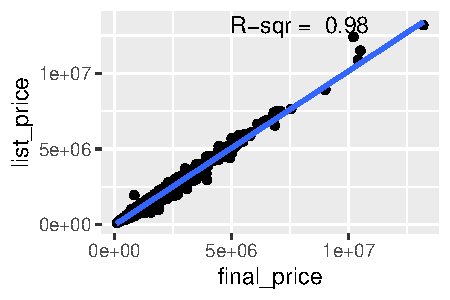
\includegraphics{R-markdown_sean_files/figure-latex/final list-1} 

}

\caption{Final Price vs. List Price\label{sec:fig6}}\label{fig:final list}
\end{figure}
\newpage

\hypertarget{modeling-1}{%
\subsection{Modeling}\label{modeling-1}}

The k-fold cross-validation method evaluates the model performance on
different subsets of the training data calculates the average prediction
error rate. We used k = 10 for our project,and this method was used
instead of the simple train-test-split as it gives a more valid
estimation of model effectiveness.

\hypertarget{decision-tree-model}{%
\subsubsection{Decision Tree Model}\label{decision-tree-model}}

The decision tree model was tuned with different values of cp
(complexity). Value of cp = 0.00001 was found to be the optimal value.

\begin{center}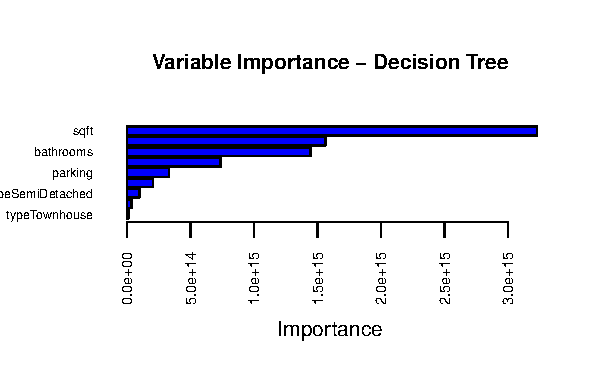
\includegraphics{R-markdown_sean_files/figure-latex/Decision Tree Model-1} \end{center}

\hypertarget{random-forest-model}{%
\subsubsection{Random Forest Model}\label{random-forest-model}}

The Random Forest was original trained with ntree = 300 and mtry = 8.
After tuning the model, ntree = 150 and mtry = 6 were used due to better
model performance.

\begin{center}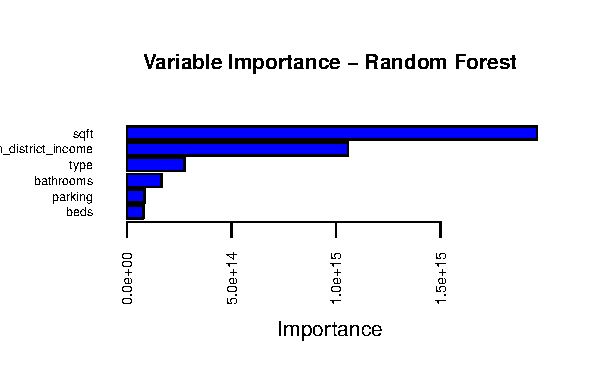
\includegraphics{R-markdown_sean_files/figure-latex/Random Forest Model-1} \end{center}

\hypertarget{gradient-boosting-model}{%
\subsubsection{Gradient Boosting Model}\label{gradient-boosting-model}}

The gradient boosting model was tuned by several different parameters.
The best performing model used the following parameters: n.trees = 200,
interaction.depth = 9, shrinkage = 0.1 and n.minobsinnode = 20.

\begin{center}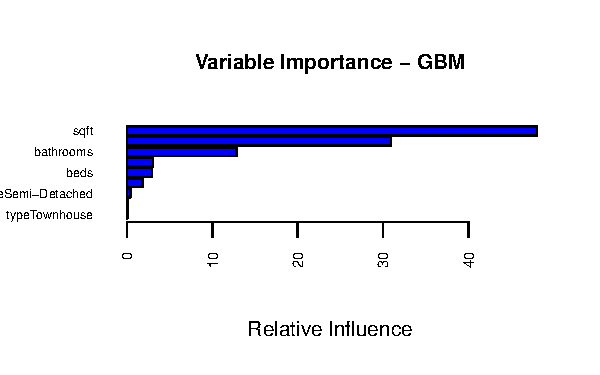
\includegraphics{R-markdown_sean_files/figure-latex/GBM importance-1} \end{center}

\hypertarget{extreme-gradient-boosting-model}{%
\subsubsection{Extreme Gradient Boosting
Model}\label{extreme-gradient-boosting-model}}

The XGBoost model was tuned with several parameters. The best performing
model used the following parameters: nrounds = 200, max\_depth = 6, eta
= 0.1, gamma = 0, colsample\_bytree = 0.8, min\_child\_weight = 5 and
subsample = 0.8.

\begin{center}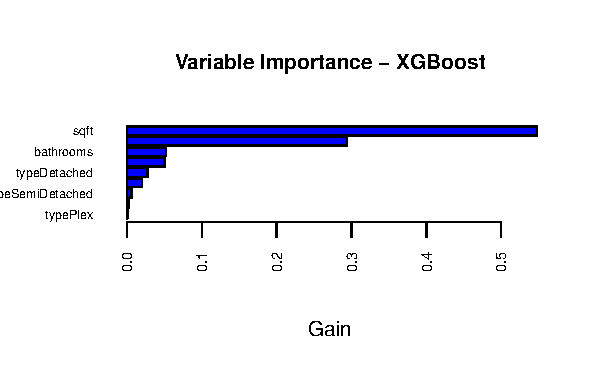
\includegraphics{R-markdown_sean_files/figure-latex/Extreme Gradient Boosting Model-1} \end{center}

\hypertarget{model-summary}{%
\subsubsection{Model Summary}\label{model-summary}}

All models found sqft and mean\_district\_income to be important
predictors of final\_price. Mean Absolute Error (MAE) tells the average
error of the variable we want to predict. Root Mean-Squared Error (RMSE)
is similar with MAE but it is more useful when we are interested in
fewer larger errors over many small errors. Overall, we prioritize model
stability and thus prioritized RMSE over MAE. \(R^2\) computes how much
better the regression fits the data than the mean line, which gives an
overall score. All the models had similar RMSE, MAE and \(R^2\). For
predicting house price, we desired a model with the lowest RMSE and MAE
to keep the high accuracy of prediction. The XGBoost model had the
highest \(R^2\) as well as the lowest RMSE and MAE, thus, it was chosen
for deployment.

\begin{longtable}[]{@{}lrrr@{}}
\caption{Model Accuracy}\tabularnewline
\toprule
model & RMSE & R2 & MAE\tabularnewline
\midrule
\endfirsthead
\toprule
model & RMSE & R2 & MAE\tabularnewline
\midrule
\endhead
decision\_tree & 274957.8 & 0.81 & 135701.0\tabularnewline
random\_forest & 233734.1 & 0.85 & 119745.2\tabularnewline
gradient\_boosting & 257316.5 & 0.83 & 134117.1\tabularnewline
extreme\_gradient\_boosting & 220850.4 & 0.86 & 116308.5\tabularnewline
\bottomrule
\end{longtable}

\hypertarget{deployment-1}{%
\subsubsection{Deployment}\label{deployment-1}}

The user interface (UI) contains a map of Toronto for geographic
navigation and also allows the user to select various inputs to predict
property price. While the user would choose a district of interest from
the front end, the back end links the district chosen with income and
uses mean\_district\_income as the model input instead. We chose to use
XGBoost, since it was the most accurate model as the back-end for our
application.

\hypertarget{discussion}{%
\section{Discussion}\label{discussion}}

Our project applied several non-parametric machine learning algorithms
to predict Toronto house prices. We cleaned the dataset by imputing
missing values using the CART algorithm from MICE. We then tuned each
model with cross-validation of k=10 using gridSearch. Overall, we found
the XGBoost model to be the most accurate, with an RMSE of 220850.4, an
\(R^2\) of 0.83, and a MAE of 116308.5. We then used R Shiny to deploy
our application with XGBoost as the predictive back-end. The application
can aid both potential Toronto home buyers and sellers in making
purchasing decisions, whether it's by validating list prices or
predicting final prices.

Our study does come with several limitations. First, the dataset only
ranged from 2018 to 2019 and is now likely to be dated. The Toronto
housing market had seen incredible growth over the past few years. While
the recent advent of the COVID-19 pandemic has led to a steep decline in
both listings and sales by 41\% and 48\% respectively, prices are still
forecasted to grow by 5\% year-over-year {[}15{]}{[}16{]}{[}17{]}.
Therefore, the model will need to be re-trained and re-evaluated on new
data. A second limitation is that we had to imputed missing values for
sqft. While MICE is a robust package for imputing missing data, it may
nevertheless introduce additional bias. Third, we believe there are
other important features that were not captured in our model, such as
proximity to nature, accessibility to public transit, and renovations
and amenities - to name a few. To increase the potential accuracy of our
model, the current dataset would ideally be linked with other sources of
data.

\hypertarget{ethical-considerations}{%
\subsection{Ethical Considerations}\label{ethical-considerations}}

There are strong financial incentives associated with purchasing
property. ``All models are wrong, but some are useful'' is a common
saying within the statistics and data science community. As even our
most accurate model is still prone to an average error of around
\$100,000, blindly trusting the model without consulting other sources
of knowledge may result in highly unprofitable decisions. As such, we
hope that the application serves mostly as a proof-of-concept rather
than a robust money-making tool. Nevertheless, we still found certain
factors, such as square footage and mean-district income, to be salient
predictors of housing price.

Another ethical concern might be that the application can be used as an
easily accessible method for estimating wealth. Out of sheer curiosity
(or perhaps out of malicious intent), a user may use the application to
predict the house prices of unsuspecting strangers, neighbors, or family
members. While one might be able to generate a reasonable price estimate
based on intuition, research, or subject matter expertise, the
application provides an near-instantaneous calculation. Should the model
become highly accurate, then the application could lead to abuse by any
number of interested stakeholders, such as banks, private loaners, or
criminals. Therefore, regulations on application usage might be
implemented, such as allowing access to only trusted institutions with
an acceptable use. An example of such would be to allow a realtor to
predict a listing price before putting a house up for sale.

We also worry that the widespread use of such a deterministic
application will negatively impact free-market dynamics within housing
ecosystems. Would growth stagnate if prices are pre-determined by a
machine-learning algorithm? Of course, we expect that buyers and sellers
will try to `play the system' - but that can lead to another caveat
where injustice is created by accessibility. If the app is under
regulation, that could still lead to abuse from institutional players.
An interesting comparison might be to the investing community, where
apps such as Robinhood or Wealthsimple have massively created
accessibility to the stock market for individual investors. However,
research has shown that individual investors on average under-perform
both professional traders and the market at large {[}18{]}. Therefore,
any app that claims to generate deep financial incentives ought to
properly inform its users of the potential risks.

\hypertarget{acknowledgements}{%
\section{Acknowledgements}\label{acknowledgements}}

The authors would like to thank Hashmat Rohian, adjunct faculty at York
University for supervision of the project. We also thank Slava Spirin
for the original extraction of the Toronto Housing dataset {[}2{]}.
Finally, we thank Steve V. Miller for creation of the manuscript
template in R Markdown {[}19{]}.

\newpage

\hypertarget{references}{%
\section{References}\label{references}}

\noindent

\hypertarget{refs}{}
\leavevmode\hypertarget{ref-noauthor_house_nodate}{}%
1. House price index -- developed by teranet in alliance with national
bank of canada Available at: \url{https://housepriceindex.ca/}
{[}Accessed November 1, 2020{]}.

\leavevmode\hypertarget{ref-spirin_slavaspirintoronto-housing-price-prediction_2020}{}%
2. Spirin, S. (2020). Slavaspirin/toronto-housing-price-prediction
Available at:
\url{https://github.com/slavaspirin/Toronto-housing-price-prediction}
{[}Accessed October 26, 2020{]}.

\leavevmode\hypertarget{ref-ayilara_impact_2019}{}%
3. Ayilara, O.F., Zhang, L., Sajobi, T.T., Sawatzky, R., Bohm, E., and
Lix, L.M. (2019). Impact of missing data on bias and precision when
estimating change in patient-reported outcomes from a clinical registry.
Health and Quality of Life Outcomes \emph{17}, 106. Available at:
\url{https://doi.org/10.1186/s12955-019-1181-2} {[}Accessed November 1,
2020{]}.

\leavevmode\hypertarget{ref-rubin_inference_1976}{}%
4. Rubin, D.B. (1976). Inference and missing data. Biometrika \emph{63},
581--592. Available at:
\url{https://academic.oup.com/biomet/article/63/3/581/270932}
{[}Accessed November 1, 2020{]}.

\leavevmode\hypertarget{ref-noauthor_quickly_nodate}{}%
5. Quickly create elegant regression results tables and plots when
modelling Available at: \url{https://finalfit.org/} {[}Accessed November
1, 2020{]}.

\leavevmode\hypertarget{ref-noauthor_mice_nodate}{}%
6. Mice function r documentation Available at:
\url{https://www.rdocumentation.org/packages/mice/versions/3.11.0/topics/mice}
{[}Accessed November 1, 2020{]}.

\leavevmode\hypertarget{ref-kumar_machine_2020}{}%
7. Kumar, P., Sinha, K., Nere, N.K., Shin, Y., Ho, R., Mlinar, L.B., and
Sheikh, A.Y. (2020). A machine learning framework for computationally
expensive transient models. Scientific Reports \emph{10}, 11492.
Available at: \url{https://www.nature.com/articles/s41598-020-67546-w}
{[}Accessed November 1, 2020{]}.

\leavevmode\hypertarget{ref-casson_understanding_2014}{}%
8. Casson, R.J., and Farmer, L.D. (2014). Understanding and checking the
assumptions of linear regression: A primer for medical researchers.
Clinical \& Experimental Ophthalmology \emph{42}, 590--596. Available
at: \url{https://onlinelibrary.wiley.com/doi/abs/10.1111/ceo.12358}
{[}Accessed November 1, 2020{]}.

\leavevmode\hypertarget{ref-noauthor_rpart_nodate}{}%
9. Rpart function r documentation Available at:
\url{https://www.rdocumentation.org/packages/rpart/versions/4.1-15/topics/rpart}
{[}Accessed November 1, 2020{]}.

\leavevmode\hypertarget{ref-noauthor_randomforest_nodate}{}%
10. randomForest function r documentation Available at:
\url{https://www.rdocumentation.org/packages/randomForest/versions/4.6-14/topics/randomForest}
{[}Accessed November 1, 2020{]}.

\leavevmode\hypertarget{ref-noauthor_gbm_nodate}{}%
11. Gbm function r documentation Available at:
\url{https://www.rdocumentation.org/packages/gbm/versions/1.1-1/topics/gbm}
{[}Accessed November 1, 2020{]}.

\leavevmode\hypertarget{ref-noauthor_xgboost_nodate}{}%
12. Xgboost package r documentation Available at:
\url{https://www.rdocumentation.org/packages/xgboost/versions/0.4-4}
{[}Accessed November 1, 2020{]}.

\leavevmode\hypertarget{ref-noauthor_explore_nodate}{}%
13. Explore the city of toronto - we're the neighbourhood guide.
Neighbourhood guide Available at:
\url{https://www.neighbourhoodguide.com/toronto/} {[}Accessed November
1, 2020{]}.

\leavevmode\hypertarget{ref-noauthor_neighbourhood_2017}{}%
14. Neighbourhood profiles. City of toronto (2017). Available at:
\url{https://www.toronto.ca/city-government/data-research-maps/neighbourhoods-communities/neighbourhood-profiles/}
{[}Accessed November 1, 2020{]}.

\leavevmode\hypertarget{ref-noauthor_housing-market-insight-toronto-cma_nodate}{}%
15. Housing-market-insight-toronto-CMA Available at:
\url{https://www.cmhc-schl.gc.ca/en/data-and-research/publications-and-reports/housing-market-insight-toronto-cma}
{[}Accessed November 1, 2020{]}.

\leavevmode\hypertarget{ref-mcnutt_toronto_2020}{}%
16. McNutt, L. (2020). Toronto housing market outlook (fall 2020) RE/MAX
canada news. RE/MAX canada. Available at:
\url{https://blog.remax.ca/toronto-housing-market-outlook/} {[}Accessed
November 1, 2020{]}.

\leavevmode\hypertarget{ref-noauthor_housing_nodate}{}%
17. Housing market assessment Available at:
\url{https://www.cmhc-schl.gc.ca/en/data-and-research/publications-and-reports/housing-market-assessment}
{[}Accessed November 1, 2020{]}.

\leavevmode\hypertarget{ref-barber_chapter_2013}{}%
18. Barber, B.M., and Odean, T. (2013). Chapter 22 - the behavior of
individual investors. In Handbook of the economics of finance, G. M.
Constantinides, M. Harris, and R. M. Stulz, eds. (Elsevier), pp.
1533--1570. Available at:
\url{http://www.sciencedirect.com/science/article/pii/B9780444594068000226}
{[}Accessed November 1, 2020{]}.

\leavevmode\hypertarget{ref-miller_r_nodate}{}%
19. Miller, S.V. An r markdown template for academic manuscripts. Steven
v. Miller. Available at:
\url{http://svmiller.com/blog/2016/02/svm-r-markdown-manuscript/}
{[}Accessed October 26, 2020{]}.





\newpage
\singlespacing 
\end{document}
